\documentclass[14pt,a4paper]{article}

\usepackage[utf8]{inputenc}

\usepackage{amssymb}

\usepackage{amsfonts}


\usepackage{graphicx}

\usepackage[left=3cm,right=3cm,top=3cm,bottom=3cm]{geometry}

\date{\today}


\begin{document}
\title{Comunicación para el desarrollo del proyecto}


\includegraphics[scale=0.4]{uv1.png} 
\author{Equipo 1}


\section{Objetivos}
\begin{itemize}
\item \textit{Establecer los distintos roles.}
\item \textit{Cumplir con los objetivos establecidos para éste proyecto.}
\item \textit{Establecer reglas para el trabajo en equipo}
\item \textit{Una comunicación éxitosa entre los miembros del equipo.}
\item \textit{Realizar llamadas para aclarar dudas.}
\end{itemize}
\vspace{0.7 cm} 



\section{Plan de comunicación}
\vspace{0.5 cm}
\begin{verse}
Para el desarrollo de este proyecto decidimos utilizar Discord porque Discord te ofrece la posibilidad de crear un sitio seguro y confiable en el cual te puedas expresar libremente. Tu servidor de Discord es tu espacio, que compartes solo con la gente especial a la que invitas. Los canales de voz de tu servidor están diseñados para que puedas unirte y salir de las conversaciones por voz y vídeo a lo largo del día. La importancia de la comunicación radica en que es nuestro medio para entendernos los unos a los otros, es nuestra herramienta para conseguir lo que necesitamos y lo que queremos, así cómo lo que somos. 
Al utilizar una herramienta de comunicación con la que todos los integrantes del equipo estaban familiarizados, fue más sencillo la distribución, así como la creación del proyecto. La elección de la plataforma adecuada jugó un papel importante en el desarrollo del proyecto, ya que gracias a ello pudimos programar nuestras reuniones, así como también dar una retroalimentación a quien tuviera alguna duda. Todos los días nos contactábamos para mantener al tanto de nuestro progreso a todos los integrantes del equipo.
\begin{figure}[htb]


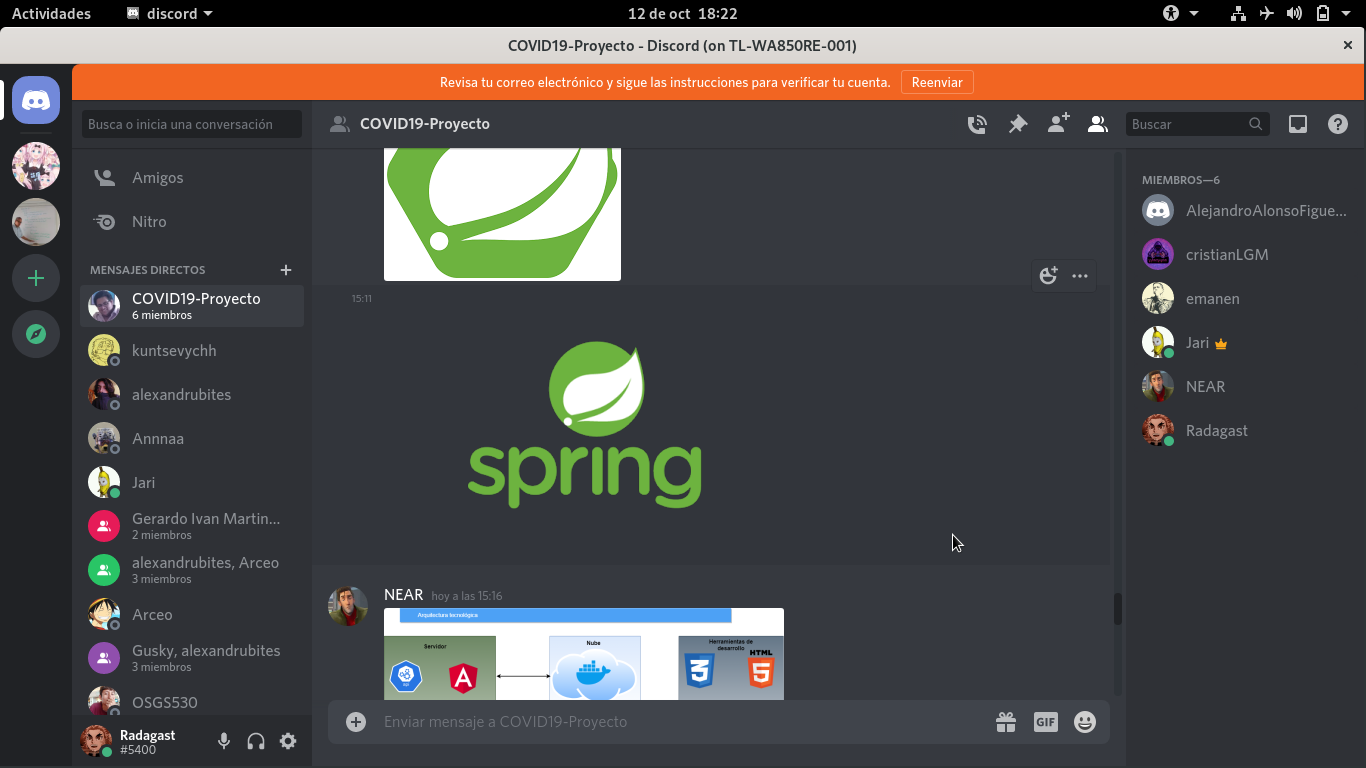
\includegraphics[scale=0.3]{Captura de pantalla de 2020-10-12 18-22-20.png} 

\caption{Captura de pantalla de nuestro grupo de Discord}
\label{fig:captura}
\end{figure}

\end{verse}
 

\end{document}